\documentclass[a4paper]{book}
\usepackage{makeidx}
\usepackage{natbib}
\usepackage{graphicx}
\usepackage{multicol}
\usepackage{float}
\usepackage{listings}
\usepackage{color}
\usepackage{ifthen}
\usepackage[table]{xcolor}
\usepackage{textcomp}
\usepackage{alltt}
\usepackage{ifpdf}
\ifpdf
\usepackage[pdftex,
            pagebackref=true,
            colorlinks=true,
            linkcolor=blue,
            unicode
           ]{hyperref}
\else
\usepackage[ps2pdf,
            pagebackref=true,
            colorlinks=true,
            linkcolor=blue,
            unicode
           ]{hyperref}
\usepackage{pspicture}
\fi
\usepackage[utf8]{inputenc}
\usepackage{mathptmx}
\usepackage[scaled=.90]{helvet}
\usepackage{courier}
\usepackage{sectsty}
\usepackage[titles]{tocloft}
\usepackage{doxygen}
\lstset{language=C++,inputencoding=utf8,basicstyle=\footnotesize,breaklines=true,breakatwhitespace=true,tabsize=4,numbers=left }
\makeindex
\setcounter{tocdepth}{3}
\renewcommand{\footrulewidth}{0.4pt}
\renewcommand{\familydefault}{\sfdefault}
\hfuzz=15pt
\setlength{\emergencystretch}{15pt}
\hbadness=750
\tolerance=750
\begin{document}
\hypersetup{pageanchor=false,citecolor=blue}
\begin{titlepage}
\vspace*{7cm}
\begin{center}
{\Large \-Blood\-Pressure\-Checker \\[1ex]\large 0.\-1\-Alpha }\\
\vspace*{1cm}
{\large \-Generated by Doxygen 1.7.6.1}\\
\vspace*{0.5cm}
{\small Thu Jun 14 2012 18:34:21}\\
\end{center}
\end{titlepage}
\clearemptydoublepage
\pagenumbering{roman}
\tableofcontents
\clearemptydoublepage
\pagenumbering{arabic}
\hypersetup{pageanchor=true,citecolor=blue}
\chapter{\-Todo \-List}
\label{todo}
\hypertarget{todo}{}

\begin{DoxyRefList}
\item[\label{todo__todo000001}%
\hypertarget{todo__todo000001}{}%
File \hyperlink{Backpack_8py}{Backpack.py} ]Modul\-: reading and interpreting mysql configuration 

Modul\-: create intial mysql db 

Modul\-: insert, update and read data from db 

Modul\-: saves extracted data as P\-D\-F  
\item[\label{todo__todo000002}%
\hypertarget{todo__todo000002}{}%
Global \hyperlink{classcalc__ep_1_1MainWindow_a784d15d1157ea5b181c63d73daa3fc5e}{Main\-Window.help\-Handbook} ]this needs to be implemented  
\item[\label{todo__todo000003}%
\hypertarget{todo__todo000003}{}%
Global \hyperlink{classgui_1_1window_1_1MainWindow_a784d15d1157ea5b181c63d73daa3fc5e}{Main\-Window.help\-Handbook} ]this needs to be implemented  
\item[\label{todo__todo000011}%
\hypertarget{todo__todo000011}{}%
Global \hyperlink{classgui_1_1window2_1_1MainWindow_a784d15d1157ea5b181c63d73daa3fc5e}{Main\-Window.help\-Handbook} ]this needs to be implemented  
\item[\label{todo__todo000024}%
\hypertarget{todo__todo000024}{}%
Global \hyperlink{classgui_1_1window3_1_1MenuWin_ab66f1da42371ac6f08a9817adf59a38e}{Menu\-Win.add\-Help} ]\-: add additional help contexts -\/ maybe even a real {\itshape context} {\itshape help}  
\item[\label{todo__todo000026}%
\hypertarget{todo__todo000026}{}%
Global \hyperlink{classgui_1_1window3_1_1MenuWin_a4b810e6adc7d147eaa8edb45dd5891ca}{Menu\-Win.context\-Help} ]\-: Implement a context help method  
\item[\label{todo__todo000025}%
\hypertarget{todo__todo000025}{}%
Global \hyperlink{classgui_1_1window3_1_1MenuWin_a2e91f76cce6e9b7a03830202f45aecf0}{Menu\-Win.first\-Steps} ]\-: implement this help method 

\-: write the first step howtos...  
\item[\label{todo__todo000028}%
\hypertarget{todo__todo000028}{}%
Namespace \hyperlink{namespacetoolbox}{toolbox} ]Create the modules for Python 3.\-x  
\item[\label{todo__todo000030}%
\hypertarget{todo__todo000030}{}%
File \hyperlink{xmlbox_8py}{xmlbox.py} ]There have be a clean out and a unifying of dictionary keys... 
\end{DoxyRefList}
\chapter{\-Data \-Structure \-Index}
\section{Class Hierarchy}
This inheritance list is sorted roughly, but not completely, alphabetically\-:\begin{DoxyCompactList}
\item \contentsline{section}{adamant\-X\-M\-L}{\pageref{classrpgtoolbox_1_1errbox_1_1adamantXML}}{}
\item \contentsline{section}{adamant\-X\-M\-L}{\pageref{classrpgToolDefinitions_1_1toolbox_1_1errbox_1_1adamantXML}}{}
\item \contentsline{section}{Auto\-Scrollbar}{\pageref{classgui_1_1winhelper_1_1AutoScrollbar}}{}
\item \contentsline{section}{blank\-Window}{\pageref{classgui_1_1window_1_1blankWindow}}{}
\begin{DoxyCompactList}
\item \contentsline{section}{Main\-Window}{\pageref{classcalc__ep_1_1MainWindow}}{}
\item \contentsline{section}{attrib\-Win}{\pageref{classgui_1_1window_1_1attribWin}}{}
\item \contentsline{section}{conf\-Window}{\pageref{classgui_1_1window_1_1confWindow}}{}
\item \contentsline{section}{input\-Win}{\pageref{classgui_1_1window_1_1inputWin}}{}
\item \contentsline{section}{Main\-Window}{\pageref{classgui_1_1window_1_1MainWindow}}{}
\item \contentsline{section}{meta\-Win}{\pageref{classgui_1_1window_1_1metaWin}}{}
\end{DoxyCompactList}
\item \contentsline{section}{blank\-Window}{\pageref{classgui_1_1window2_1_1blankWindow}}{}
\begin{DoxyCompactList}
\item \contentsline{section}{attrib\-Meta\-Win}{\pageref{classgui_1_1window2_1_1attribMetaWin}}{}
\item \contentsline{section}{attrib\-Win}{\pageref{classgui_1_1window2_1_1attribWin}}{}
\item \contentsline{section}{conf\-Window}{\pageref{classgui_1_1window2_1_1confWindow}}{}
\item \contentsline{section}{connect\-Elem}{\pageref{classgui_1_1window2_1_1connectElem}}{}
\item \contentsline{section}{input\-Win}{\pageref{classgui_1_1window2_1_1inputWin}}{}
\item \contentsline{section}{Main\-Window}{\pageref{classgui_1_1window2_1_1MainWindow}}{}
\item \contentsline{section}{meta\-Win}{\pageref{classgui_1_1window2_1_1metaWin}}{}
\end{DoxyCompactList}
\item \contentsline{section}{chk\-Cfg}{\pageref{classrpgtoolbox_1_1confbox_1_1chkCfg}}{}
\item \contentsline{section}{chk\-Cfg}{\pageref{classrpgToolDefinitions_1_1toolbox_1_1confbox_1_1chkCfg}}{}
\item \contentsline{section}{draw\-Tree}{\pageref{classgui_1_1window2_1_1drawTree}}{}
\item \contentsline{section}{handle\-X\-M\-L}{\pageref{classrpgToolDefinitions_1_1toolbox_1_1xmltools_1_1handleXML}}{}
\item \contentsline{section}{Info\-Canvas}{\pageref{classgui_1_1winhelper_1_1InfoCanvas}}{}
\item \contentsline{section}{Magic}{\pageref{classrpgToolDefinitions_1_1MERSTables_1_1Magic}}{}
\item \contentsline{section}{Menu\-Win}{\pageref{classgui_1_1window3_1_1MenuWin}}{}
\item \contentsline{section}{message\-Window}{\pageref{classgui_1_1window_1_1messageWindow}}{}
\item \contentsline{section}{message\-Window}{\pageref{classgui_1_1window2_1_1messageWindow}}{}
\item \contentsline{section}{message\-Window}{\pageref{classgui_1_1window3_1_1messageWindow}}{}
\item \contentsline{section}{My\-Class}{\pageref{classrpgToolDefinitions_1_1RMTables_1_1MyClass}}{}
\end{DoxyCompactList}

\chapter{\-Data \-Structure \-Index}
\section{Data Structures}
Here are the data structures with brief descriptions\-:\begin{DoxyCompactList}
\item\contentsline{section}{\hyperlink{classrpgtoolbox_1_1errbox_1_1adamantXML}{adamant\-X\-M\-L} \\*Objects of this class will be raised in case of errors with X\-M\-L files used for A\-Da\-Mant }{\pageref{classrpgtoolbox_1_1errbox_1_1adamantXML}}{}
\item\contentsline{section}{\hyperlink{classrpgToolDefinitions_1_1toolbox_1_1errbox_1_1adamantXML}{adamant\-X\-M\-L} \\*Objects of this class will be raised in case of errors with X\-M\-L files used for A\-Da\-Mant }{\pageref{classrpgToolDefinitions_1_1toolbox_1_1errbox_1_1adamantXML}}{}
\item\contentsline{section}{\hyperlink{classgui_1_1window2_1_1attribMetaWin}{attrib\-Meta\-Win} \\*This opens a window for setting the attributes of meta data fields }{\pageref{classgui_1_1window2_1_1attribMetaWin}}{}
\item\contentsline{section}{\hyperlink{classgui_1_1window_1_1attribWin}{attrib\-Win} \\*This generates a window where attributes can be added to chosen elements of structure }{\pageref{classgui_1_1window_1_1attribWin}}{}
\item\contentsline{section}{\hyperlink{classgui_1_1window2_1_1attribWin}{attrib\-Win} \\*This generates a window where attributes can be added to chosen elements of structure }{\pageref{classgui_1_1window2_1_1attribWin}}{}
\item\contentsline{section}{\hyperlink{classgui_1_1winhelper_1_1AutoScrollbar}{Auto\-Scrollbar} \\*A scrollbar that hides itself if it's not needed }{\pageref{classgui_1_1winhelper_1_1AutoScrollbar}}{}
\item\contentsline{section}{\hyperlink{classgui_1_1window_1_1blankWindow}{blank\-Window} \\*A simple window class with a not filled menu bar }{\pageref{classgui_1_1window_1_1blankWindow}}{}
\item\contentsline{section}{\hyperlink{classgui_1_1window2_1_1blankWindow}{blank\-Window} \\*A simple window class with a not filled menu bar }{\pageref{classgui_1_1window2_1_1blankWindow}}{}
\item\contentsline{section}{\hyperlink{classrpgtoolbox_1_1confbox_1_1chkCfg}{chk\-Cfg} \\*These Objects reads out a given config file and store the content of the configuration in a dictionary }{\pageref{classrpgtoolbox_1_1confbox_1_1chkCfg}}{}
\item\contentsline{section}{\hyperlink{classrpgToolDefinitions_1_1toolbox_1_1confbox_1_1chkCfg}{chk\-Cfg} \\*These Objects reads out a given config file and store the content of the configuration in a dictionary }{\pageref{classrpgToolDefinitions_1_1toolbox_1_1confbox_1_1chkCfg}}{}
\item\contentsline{section}{\hyperlink{classgui_1_1window2_1_1confWindow}{conf\-Window} \\*This class builds a window for selecting and saving options of A\-Da\-Man\-T }{\pageref{classgui_1_1window2_1_1confWindow}}{}
\item\contentsline{section}{\hyperlink{classgui_1_1window_1_1confWindow}{conf\-Window} \\*This class builds a window for selecting and saving options of A\-Da\-Man\-T }{\pageref{classgui_1_1window_1_1confWindow}}{}
\item\contentsline{section}{\hyperlink{classgui_1_1window2_1_1connectElem}{connect\-Elem} \\*This creates a window to connect elements of structure logically }{\pageref{classgui_1_1window2_1_1connectElem}}{}
\item\contentsline{section}{\hyperlink{classgui_1_1window2_1_1drawTree}{draw\-Tree} \\*This class creates an object to draw a graph of a tree structure (in a dictionary) }{\pageref{classgui_1_1window2_1_1drawTree}}{}
\item\contentsline{section}{\hyperlink{classrpgToolDefinitions_1_1toolbox_1_1xmltools_1_1handleXML}{handle\-X\-M\-L} \\*This class offers methods to convert dictionaries to X\-M\-L and back }{\pageref{classrpgToolDefinitions_1_1toolbox_1_1xmltools_1_1handleXML}}{}
\item\contentsline{section}{\hyperlink{classgui_1_1winhelper_1_1InfoCanvas}{Info\-Canvas} \\*A Canvas-\/widget that holds a scrollable Message-\/widget }{\pageref{classgui_1_1winhelper_1_1InfoCanvas}}{}
\item\contentsline{section}{\hyperlink{classgui_1_1window_1_1inputWin}{input\-Win} \\*Objects of this class type are windows for input the wanted data structure }{\pageref{classgui_1_1window_1_1inputWin}}{}
\item\contentsline{section}{\hyperlink{classgui_1_1window2_1_1inputWin}{input\-Win} \\*Objects of this class type are windows for input the wanted data structure }{\pageref{classgui_1_1window2_1_1inputWin}}{}
\item\contentsline{section}{\hyperlink{classrpgToolDefinitions_1_1MERSTables_1_1Magic}{Magic} \\*Classdocs }{\pageref{classrpgToolDefinitions_1_1MERSTables_1_1Magic}}{}
\item\contentsline{section}{\hyperlink{classgui_1_1window_1_1MainWindow}{Main\-Window} \\*This is the class for the main window object }{\pageref{classgui_1_1window_1_1MainWindow}}{}
\item\contentsline{section}{\hyperlink{classcalc__ep_1_1MainWindow}{Main\-Window} \\*This is the class for the main window object }{\pageref{classcalc__ep_1_1MainWindow}}{}
\item\contentsline{section}{\hyperlink{classgui_1_1window2_1_1MainWindow}{Main\-Window} \\*This is the class for the main window object }{\pageref{classgui_1_1window2_1_1MainWindow}}{}
\item\contentsline{section}{\hyperlink{classgui_1_1window3_1_1MenuWin}{Menu\-Win} \\*Master class for all windows using menus }{\pageref{classgui_1_1window3_1_1MenuWin}}{}
\item\contentsline{section}{\hyperlink{classgui_1_1window_1_1messageWindow}{message\-Window} \\*A class to build a message window containing version, author and email on default }{\pageref{classgui_1_1window_1_1messageWindow}}{}
\item\contentsline{section}{\hyperlink{classgui_1_1window2_1_1messageWindow}{message\-Window} \\*A class to build a message window containing version, author and email on default }{\pageref{classgui_1_1window2_1_1messageWindow}}{}
\item\contentsline{section}{\hyperlink{classgui_1_1window3_1_1messageWindow}{message\-Window} \\*A class to build a message window containing version, author and email on default }{\pageref{classgui_1_1window3_1_1messageWindow}}{}
\item\contentsline{section}{\hyperlink{classgui_1_1window_1_1metaWin}{meta\-Win} \\*Creates a window for generating meta data fields }{\pageref{classgui_1_1window_1_1metaWin}}{}
\item\contentsline{section}{\hyperlink{classgui_1_1window2_1_1metaWin}{meta\-Win} \\*Creates a window for generating meta data fields }{\pageref{classgui_1_1window2_1_1metaWin}}{}
\item\contentsline{section}{\hyperlink{classrpgToolDefinitions_1_1RMTables_1_1MyClass}{My\-Class} \\*Created on 13.\-12.\-2015 }{\pageref{classrpgToolDefinitions_1_1RMTables_1_1MyClass}}{}
\end{DoxyCompactList}

\chapter{\-File \-Index}
\section{\-File \-List}
\-Here is a list of all documented files with brief descriptions\-:\begin{DoxyCompactList}
\item\contentsline{section}{\hyperlink{language_8py}{language.\-py} }{\pageref{language_8py}}{}
\item\contentsline{section}{\hyperlink{logtools_8py}{logtools.\-py} }{\pageref{logtools_8py}}{}
\item\contentsline{section}{\hyperlink{ostools_8py}{ostools.\-py} }{\pageref{ostools_8py}}{}
\end{DoxyCompactList}

\chapter{\-Data \-Structure \-Documentation}
\hypertarget{classgui_1_1window2_1_1blankWindow}{\section{blank\-Window Class Reference}
\label{classgui_1_1window2_1_1blankWindow}\index{blank\-Window@{blank\-Window}}
}


A simple window class with a not filled menu bar.  




Inheritance diagram for blank\-Window\-:\nopagebreak
\begin{figure}[H]
\begin{center}
\leavevmode
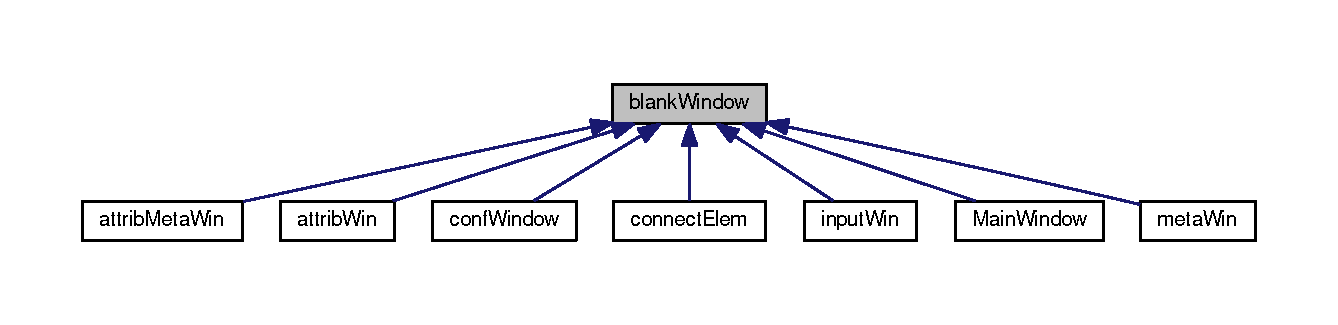
\includegraphics[width=350pt]{classgui_1_1window2_1_1blankWindow__inherit__graph}
\end{center}
\end{figure}
\subsection*{Public Member Functions}
\begin{DoxyCompactItemize}
\item 
\hypertarget{classgui_1_1window2_1_1blankWindow_a615f3073891733337c33f599f89ec7ef}{def \hyperlink{classgui_1_1window2_1_1blankWindow_a615f3073891733337c33f599f89ec7ef}{notdoneyet}}\label{classgui_1_1window2_1_1blankWindow_a615f3073891733337c33f599f89ec7ef}

\begin{DoxyCompactList}\small\item\em a simple dummy method for not yet implemented methods \end{DoxyCompactList}\end{DoxyCompactItemize}


\subsection{Detailed Description}
A simple window class with a not filled menu bar. 


\begin{DoxyParams}{Parameters}
{\em lang} & chosen language for the menu. \\
\hline
\end{DoxyParams}


The documentation for this class was generated from the following file\-:\begin{DoxyCompactItemize}
\item 
\hyperlink{window2_8py}{window2.\-py}\end{DoxyCompactItemize}

\hypertarget{classgui_1_1window2_1_1mainWindow}{\section{main\-Window \-Class \-Reference}
\label{classgui_1_1window2_1_1mainWindow}\index{main\-Window@{main\-Window}}
}


\-This class generates the main window of the program.  


\-Inheritance diagram for main\-Window\-:\begin{figure}[H]
\begin{center}
\leavevmode
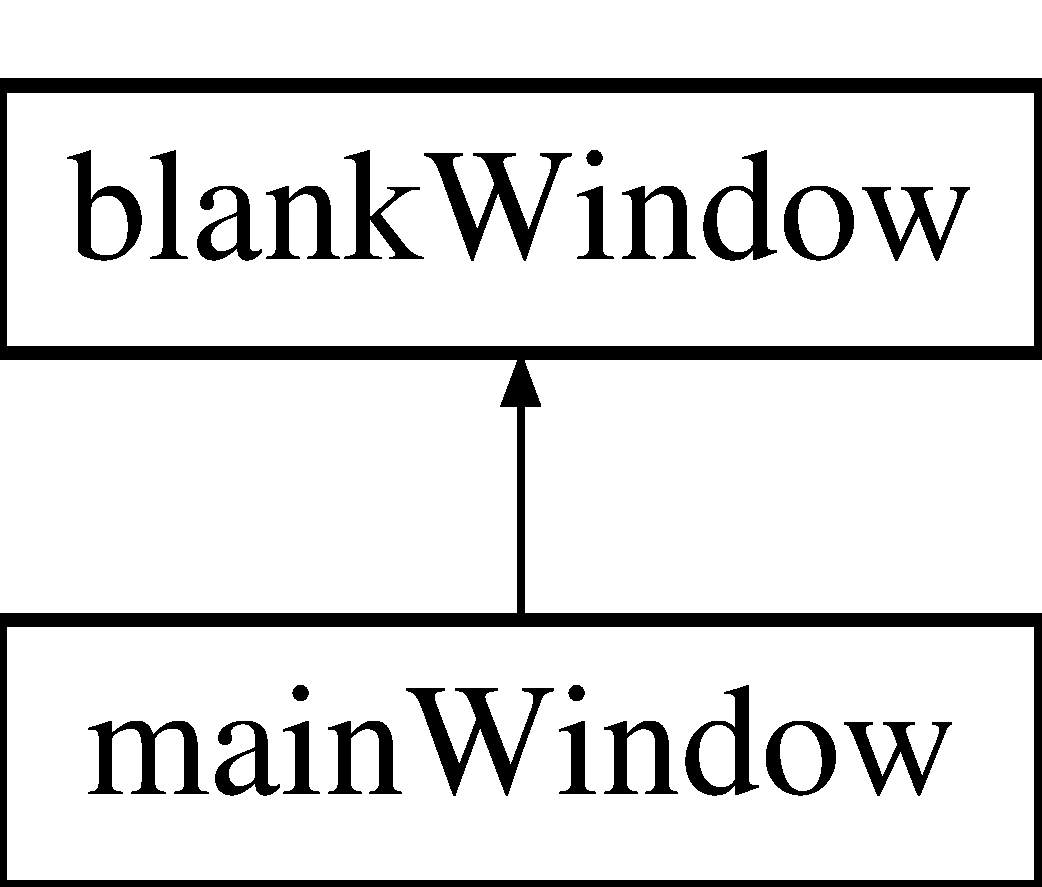
\includegraphics[height=2.000000cm]{classgui_1_1window2_1_1mainWindow}
\end{center}
\end{figure}
\subsection*{\-Private \-Member \-Functions}
\begin{DoxyCompactItemize}
\item 
\hypertarget{classgui_1_1window2_1_1mainWindow_aba31902186de9c54cc3cba810c1f3634}{def \hyperlink{classgui_1_1window2_1_1mainWindow_aba31902186de9c54cc3cba810c1f3634}{\-\_\-add\-File\-Menu}}\label{classgui_1_1window2_1_1mainWindow_aba31902186de9c54cc3cba810c1f3634}

\begin{DoxyCompactList}\small\item\em \-This method adds a \-File menu to the windows menu bar. \end{DoxyCompactList}\item 
def \hyperlink{classgui_1_1window2_1_1mainWindow_ab88021b976d074d30b5fdc8561f72192}{\-\_\-new\-File}
\begin{DoxyCompactList}\small\item\em \-This generates a new file. \end{DoxyCompactList}\item 
def \hyperlink{classgui_1_1window2_1_1mainWindow_ac47f719d35c8244134cff4710a4d249a}{\-\_\-open\-File}
\begin{DoxyCompactList}\small\item\em \-This opens a file. \end{DoxyCompactList}\item 
def \hyperlink{classgui_1_1window2_1_1mainWindow_a1d1d8399c211ab2c39ead212fa6c8407}{\-\_\-save\-File}
\begin{DoxyCompactList}\small\item\em \-This saves the data into a file. \end{DoxyCompactList}\item 
def \hyperlink{classgui_1_1window2_1_1mainWindow_a1ffc3abf49be025d4db556ac63a17399}{\-\_\-save\-File\-As}
\begin{DoxyCompactList}\small\item\em \-Save data in another file. \end{DoxyCompactList}\item 
def \hyperlink{classgui_1_1window2_1_1mainWindow_a0c149717ce106ef13e42a04055a55d57}{\-\_\-add\-Edit\-Menu}
\begin{DoxyCompactList}\small\item\em \-This adds the edit menu to the menu bar. \end{DoxyCompactList}\item 
def \hyperlink{classgui_1_1window2_1_1mainWindow_adce23e84928f330db51647c12cf18a22}{\-\_\-add\-Data}
\begin{DoxyCompactList}\small\item\em \-This adds data to an existing data set. \end{DoxyCompactList}\item 
def \hyperlink{classgui_1_1window2_1_1mainWindow_a64c00769449e39362a38721688554e33}{\-\_\-remove\-Data}
\begin{DoxyCompactList}\small\item\em \-This removes data from the data set. \end{DoxyCompactList}\item 
def \hyperlink{classgui_1_1window2_1_1mainWindow_a04fc4444b5b361369b1bc1d4d6ad5f77}{\-\_\-edit\-Data}
\begin{DoxyCompactList}\small\item\em \-This edits data of an opened data set. \end{DoxyCompactList}\item 
\hypertarget{classgui_1_1window2_1_1mainWindow_a0f158fe2e69dc8e906ea1e93df4397fe}{def \hyperlink{classgui_1_1window2_1_1mainWindow_a0f158fe2e69dc8e906ea1e93df4397fe}{\-\_\-add\-Opt\-Menu}}\label{classgui_1_1window2_1_1mainWindow_a0f158fe2e69dc8e906ea1e93df4397fe}

\begin{DoxyCompactList}\small\item\em \-This adds an \-Options menu. \end{DoxyCompactList}\item 
def \hyperlink{classgui_1_1window2_1_1mainWindow_a6f03f407dd1c49e85437af18b46df69a}{\-\_\-basic\-Opts}
\begin{DoxyCompactList}\small\item\em \-This opens a window for basic options. \end{DoxyCompactList}\item 
def \hyperlink{classgui_1_1window2_1_1mainWindow_a145120f6dbe3e701fd55520b2cad767c}{\-\_\-graph\-Opts}
\begin{DoxyCompactList}\small\item\em \-This opens a window for graphical options. \end{DoxyCompactList}\item 
def \hyperlink{classgui_1_1window2_1_1mainWindow_a3e593c0bc9bef8082dc3d9e90498ae10}{\-\_\-output\-Opts}
\begin{DoxyCompactList}\small\item\em \-This opens a window for output options. \end{DoxyCompactList}\item 
\hypertarget{classgui_1_1window2_1_1mainWindow_a67ef40998197523b8ce51ec49aa57b94}{def \hyperlink{classgui_1_1window2_1_1mainWindow_a67ef40998197523b8ce51ec49aa57b94}{\-\_\-add\-Help\-Menu}}\label{classgui_1_1window2_1_1mainWindow_a67ef40998197523b8ce51ec49aa57b94}

\begin{DoxyCompactList}\small\item\em \-This adds the help menu to the menu bar. \end{DoxyCompactList}\item 
def \hyperlink{classgui_1_1window2_1_1mainWindow_af2014cc8d689aeb13bac00fa905b0538}{\-\_\-help\-Context}
\begin{DoxyCompactList}\small\item\em \-This adds a context menu to the help menu. \end{DoxyCompactList}\item 
def \hyperlink{classgui_1_1window2_1_1mainWindow_acc2bf9439798e939fbfbb414e6406b97}{\-\_\-read\-Cfg}
\begin{DoxyCompactList}\small\item\em \-This reads the config file (if any) automatically. \end{DoxyCompactList}\item 
def \hyperlink{classgui_1_1window2_1_1mainWindow_aa1cf74d1d90e70790e77d7865535e153}{\-\_\-plot\-Graph}
\begin{DoxyCompactList}\small\item\em \-Plotting graphs from selected data set. \end{DoxyCompactList}\end{DoxyCompactItemize}


\subsection{\-Detailed \-Description}
\-This class generates the main window of the program. 

\subsection{\-Member \-Function \-Documentation}
\hypertarget{classgui_1_1window2_1_1mainWindow_adce23e84928f330db51647c12cf18a22}{\index{gui\-::window2\-::main\-Window@{gui\-::window2\-::main\-Window}!\-\_\-add\-Data@{\-\_\-add\-Data}}
\index{\-\_\-add\-Data@{\-\_\-add\-Data}!gui::window2::mainWindow@{gui\-::window2\-::main\-Window}}
\subsubsection[{\-\_\-add\-Data}]{\setlength{\rightskip}{0pt plus 5cm}def {\bf \-\_\-add\-Data} (
\begin{DoxyParamCaption}
\item[{}]{self}
\end{DoxyParamCaption}
)\hspace{0.3cm}{\ttfamily  \mbox{[}private\mbox{]}}}}\label{classgui_1_1window2_1_1mainWindow_adce23e84928f330db51647c12cf18a22}


\-This adds data to an existing data set. 

\begin{DoxyRefDesc}{\-Todo}
\item[\hyperlink{todo__todo000006}{\-Todo}]this method has to be implemented \end{DoxyRefDesc}


\-References blank\-Window.\-\_\-notdoneyet().



\-Referenced by main\-Window.\-\_\-add\-Edit\-Menu().

\hypertarget{classgui_1_1window2_1_1mainWindow_a0c149717ce106ef13e42a04055a55d57}{\index{gui\-::window2\-::main\-Window@{gui\-::window2\-::main\-Window}!\-\_\-add\-Edit\-Menu@{\-\_\-add\-Edit\-Menu}}
\index{\-\_\-add\-Edit\-Menu@{\-\_\-add\-Edit\-Menu}!gui::window2::mainWindow@{gui\-::window2\-::main\-Window}}
\subsubsection[{\-\_\-add\-Edit\-Menu}]{\setlength{\rightskip}{0pt plus 5cm}def {\bf \-\_\-add\-Edit\-Menu} (
\begin{DoxyParamCaption}
\item[{}]{self}
\end{DoxyParamCaption}
)\hspace{0.3cm}{\ttfamily  \mbox{[}private\mbox{]}}}}\label{classgui_1_1window2_1_1mainWindow_a0c149717ce106ef13e42a04055a55d57}


\-This adds the edit menu to the menu bar. 

\begin{DoxyRefDesc}{\-Todo}
\item[\hyperlink{todo__todo000005}{\-Todo}]this method has to be implemented \end{DoxyRefDesc}


\-References main\-Window.\-\_\-add\-Data(), main\-Window.\-\_\-edit\-Data(), main\-Window.\-\_\-plot\-Graph(), main\-Window.\-\_\-remove\-Data(), main\-Window.\-editmenu, message\-Window.\-lang, blank\-Window.\-lang, main\-Window.\-lang, and blank\-Window.\-menu.

\hypertarget{classgui_1_1window2_1_1mainWindow_a6f03f407dd1c49e85437af18b46df69a}{\index{gui\-::window2\-::main\-Window@{gui\-::window2\-::main\-Window}!\-\_\-basic\-Opts@{\-\_\-basic\-Opts}}
\index{\-\_\-basic\-Opts@{\-\_\-basic\-Opts}!gui::window2::mainWindow@{gui\-::window2\-::main\-Window}}
\subsubsection[{\-\_\-basic\-Opts}]{\setlength{\rightskip}{0pt plus 5cm}def {\bf \-\_\-basic\-Opts} (
\begin{DoxyParamCaption}
\item[{}]{self}
\end{DoxyParamCaption}
)\hspace{0.3cm}{\ttfamily  \mbox{[}private\mbox{]}}}}\label{classgui_1_1window2_1_1mainWindow_a6f03f407dd1c49e85437af18b46df69a}


\-This opens a window for basic options. 

\begin{DoxyRefDesc}{\-Todo}
\item[\hyperlink{todo__todo000009}{\-Todo}]has to be implemented \end{DoxyRefDesc}


\-References main\-Window.\-cnf, message\-Window.\-lang, blank\-Window.\-lang, main\-Window.\-lang, message\-Window.\-window, blank\-Window.\-window, and main\-Window.\-window.



\-Referenced by main\-Window.\-\_\-add\-Opt\-Menu().

\hypertarget{classgui_1_1window2_1_1mainWindow_a04fc4444b5b361369b1bc1d4d6ad5f77}{\index{gui\-::window2\-::main\-Window@{gui\-::window2\-::main\-Window}!\-\_\-edit\-Data@{\-\_\-edit\-Data}}
\index{\-\_\-edit\-Data@{\-\_\-edit\-Data}!gui::window2::mainWindow@{gui\-::window2\-::main\-Window}}
\subsubsection[{\-\_\-edit\-Data}]{\setlength{\rightskip}{0pt plus 5cm}def {\bf \-\_\-edit\-Data} (
\begin{DoxyParamCaption}
\item[{}]{self}
\end{DoxyParamCaption}
)\hspace{0.3cm}{\ttfamily  \mbox{[}private\mbox{]}}}}\label{classgui_1_1window2_1_1mainWindow_a04fc4444b5b361369b1bc1d4d6ad5f77}


\-This edits data of an opened data set. 

\begin{DoxyRefDesc}{\-Todo}
\item[\hyperlink{todo__todo000008}{\-Todo}]this method has to be implemented \end{DoxyRefDesc}


\-References blank\-Window.\-\_\-notdoneyet().



\-Referenced by main\-Window.\-\_\-add\-Edit\-Menu().

\hypertarget{classgui_1_1window2_1_1mainWindow_a145120f6dbe3e701fd55520b2cad767c}{\index{gui\-::window2\-::main\-Window@{gui\-::window2\-::main\-Window}!\-\_\-graph\-Opts@{\-\_\-graph\-Opts}}
\index{\-\_\-graph\-Opts@{\-\_\-graph\-Opts}!gui::window2::mainWindow@{gui\-::window2\-::main\-Window}}
\subsubsection[{\-\_\-graph\-Opts}]{\setlength{\rightskip}{0pt plus 5cm}def {\bf \-\_\-graph\-Opts} (
\begin{DoxyParamCaption}
\item[{}]{self}
\end{DoxyParamCaption}
)\hspace{0.3cm}{\ttfamily  \mbox{[}private\mbox{]}}}}\label{classgui_1_1window2_1_1mainWindow_a145120f6dbe3e701fd55520b2cad767c}


\-This opens a window for graphical options. 

\begin{DoxyRefDesc}{\-Todo}
\item[\hyperlink{todo__todo000010}{\-Todo}]has to be implemented \end{DoxyRefDesc}


\-References main\-Window.\-cnf, message\-Window.\-lang, blank\-Window.\-lang, main\-Window.\-lang, message\-Window.\-window, blank\-Window.\-window, and main\-Window.\-window.



\-Referenced by main\-Window.\-\_\-add\-Opt\-Menu().

\hypertarget{classgui_1_1window2_1_1mainWindow_af2014cc8d689aeb13bac00fa905b0538}{\index{gui\-::window2\-::main\-Window@{gui\-::window2\-::main\-Window}!\-\_\-help\-Context@{\-\_\-help\-Context}}
\index{\-\_\-help\-Context@{\-\_\-help\-Context}!gui::window2::mainWindow@{gui\-::window2\-::main\-Window}}
\subsubsection[{\-\_\-help\-Context}]{\setlength{\rightskip}{0pt plus 5cm}def {\bf \-\_\-help\-Context} (
\begin{DoxyParamCaption}
\item[{}]{self}
\end{DoxyParamCaption}
)\hspace{0.3cm}{\ttfamily  \mbox{[}private\mbox{]}}}}\label{classgui_1_1window2_1_1mainWindow_af2014cc8d689aeb13bac00fa905b0538}


\-This adds a context menu to the help menu. 

\begin{DoxyRefDesc}{\-Todo}
\item[\hyperlink{todo__todo000012}{\-Todo}]this method has to be implemented \end{DoxyRefDesc}


\-References blank\-Window.\-\_\-notdoneyet().



\-Referenced by main\-Window.\-\_\-add\-Help\-Menu(), and opt\-Window.\-\_\-add\-Help\-Menu().

\hypertarget{classgui_1_1window2_1_1mainWindow_ab88021b976d074d30b5fdc8561f72192}{\index{gui\-::window2\-::main\-Window@{gui\-::window2\-::main\-Window}!\-\_\-new\-File@{\-\_\-new\-File}}
\index{\-\_\-new\-File@{\-\_\-new\-File}!gui::window2::mainWindow@{gui\-::window2\-::main\-Window}}
\subsubsection[{\-\_\-new\-File}]{\setlength{\rightskip}{0pt plus 5cm}def {\bf \-\_\-new\-File} (
\begin{DoxyParamCaption}
\item[{}]{self}
\end{DoxyParamCaption}
)\hspace{0.3cm}{\ttfamily  \mbox{[}private\mbox{]}}}}\label{classgui_1_1window2_1_1mainWindow_ab88021b976d074d30b5fdc8561f72192}


\-This generates a new file. 

\begin{DoxyRefDesc}{\-Todo}
\item[\hyperlink{todo__todo000001}{\-Todo}]this method has to be implemented \end{DoxyRefDesc}


\-References blank\-Window.\-\_\-notdoneyet().



\-Referenced by main\-Window.\-\_\-add\-File\-Menu().

\hypertarget{classgui_1_1window2_1_1mainWindow_ac47f719d35c8244134cff4710a4d249a}{\index{gui\-::window2\-::main\-Window@{gui\-::window2\-::main\-Window}!\-\_\-open\-File@{\-\_\-open\-File}}
\index{\-\_\-open\-File@{\-\_\-open\-File}!gui::window2::mainWindow@{gui\-::window2\-::main\-Window}}
\subsubsection[{\-\_\-open\-File}]{\setlength{\rightskip}{0pt plus 5cm}def {\bf \-\_\-open\-File} (
\begin{DoxyParamCaption}
\item[{}]{self}
\end{DoxyParamCaption}
)\hspace{0.3cm}{\ttfamily  \mbox{[}private\mbox{]}}}}\label{classgui_1_1window2_1_1mainWindow_ac47f719d35c8244134cff4710a4d249a}


\-This opens a file. 

\begin{DoxyRefDesc}{\-Todo}
\item[\hyperlink{todo__todo000002}{\-Todo}]this method has to be implemented fully \end{DoxyRefDesc}


\-References main\-Window.\-\_\-fcontent, main\-Window.\-\_\-myfile, main\-Window.\-fp, blank\-Window.\-mask, and main\-Window.\-storepath.



\-Referenced by main\-Window.\-\_\-add\-File\-Menu().

\hypertarget{classgui_1_1window2_1_1mainWindow_a3e593c0bc9bef8082dc3d9e90498ae10}{\index{gui\-::window2\-::main\-Window@{gui\-::window2\-::main\-Window}!\-\_\-output\-Opts@{\-\_\-output\-Opts}}
\index{\-\_\-output\-Opts@{\-\_\-output\-Opts}!gui::window2::mainWindow@{gui\-::window2\-::main\-Window}}
\subsubsection[{\-\_\-output\-Opts}]{\setlength{\rightskip}{0pt plus 5cm}def {\bf \-\_\-output\-Opts} (
\begin{DoxyParamCaption}
\item[{}]{self}
\end{DoxyParamCaption}
)\hspace{0.3cm}{\ttfamily  \mbox{[}private\mbox{]}}}}\label{classgui_1_1window2_1_1mainWindow_a3e593c0bc9bef8082dc3d9e90498ae10}


\-This opens a window for output options. 

\begin{DoxyRefDesc}{\-Todo}
\item[\hyperlink{todo__todo000011}{\-Todo}]has to be implemented \end{DoxyRefDesc}


\-References main\-Window.\-cnf, message\-Window.\-lang, blank\-Window.\-lang, main\-Window.\-lang, message\-Window.\-window, blank\-Window.\-window, and main\-Window.\-window.



\-Referenced by main\-Window.\-\_\-add\-Opt\-Menu().

\hypertarget{classgui_1_1window2_1_1mainWindow_aa1cf74d1d90e70790e77d7865535e153}{\index{gui\-::window2\-::main\-Window@{gui\-::window2\-::main\-Window}!\-\_\-plot\-Graph@{\-\_\-plot\-Graph}}
\index{\-\_\-plot\-Graph@{\-\_\-plot\-Graph}!gui::window2::mainWindow@{gui\-::window2\-::main\-Window}}
\subsubsection[{\-\_\-plot\-Graph}]{\setlength{\rightskip}{0pt plus 5cm}def {\bf \-\_\-plot\-Graph} (
\begin{DoxyParamCaption}
\item[{}]{self}
\end{DoxyParamCaption}
)\hspace{0.3cm}{\ttfamily  \mbox{[}private\mbox{]}}}}\label{classgui_1_1window2_1_1mainWindow_aa1cf74d1d90e70790e77d7865535e153}


\-Plotting graphs from selected data set. 

\begin{DoxyRefDesc}{\-Todo}
\item[\hyperlink{todo__todo000014}{\-Todo}]has to be implemented fully \end{DoxyRefDesc}


\-References blank\-Window.\-\_\-notdoneyet().



\-Referenced by main\-Window.\-\_\-add\-Edit\-Menu().

\hypertarget{classgui_1_1window2_1_1mainWindow_acc2bf9439798e939fbfbb414e6406b97}{\index{gui\-::window2\-::main\-Window@{gui\-::window2\-::main\-Window}!\-\_\-read\-Cfg@{\-\_\-read\-Cfg}}
\index{\-\_\-read\-Cfg@{\-\_\-read\-Cfg}!gui::window2::mainWindow@{gui\-::window2\-::main\-Window}}
\subsubsection[{\-\_\-read\-Cfg}]{\setlength{\rightskip}{0pt plus 5cm}def {\bf \-\_\-read\-Cfg} (
\begin{DoxyParamCaption}
\item[{}]{self}
\end{DoxyParamCaption}
)\hspace{0.3cm}{\ttfamily  \mbox{[}private\mbox{]}}}}\label{classgui_1_1window2_1_1mainWindow_acc2bf9439798e939fbfbb414e6406b97}


\-This reads the config file (if any) automatically. 

\begin{DoxyRefDesc}{\-Todo}
\item[\hyperlink{todo__todo000013}{\-Todo}]has to be implemented fully \end{DoxyRefDesc}


\-References main\-Window.\-cnf.

\hypertarget{classgui_1_1window2_1_1mainWindow_a64c00769449e39362a38721688554e33}{\index{gui\-::window2\-::main\-Window@{gui\-::window2\-::main\-Window}!\-\_\-remove\-Data@{\-\_\-remove\-Data}}
\index{\-\_\-remove\-Data@{\-\_\-remove\-Data}!gui::window2::mainWindow@{gui\-::window2\-::main\-Window}}
\subsubsection[{\-\_\-remove\-Data}]{\setlength{\rightskip}{0pt plus 5cm}def {\bf \-\_\-remove\-Data} (
\begin{DoxyParamCaption}
\item[{}]{self}
\end{DoxyParamCaption}
)\hspace{0.3cm}{\ttfamily  \mbox{[}private\mbox{]}}}}\label{classgui_1_1window2_1_1mainWindow_a64c00769449e39362a38721688554e33}


\-This removes data from the data set. 

\begin{DoxyRefDesc}{\-Todo}
\item[\hyperlink{todo__todo000007}{\-Todo}]this method has to be implemented \end{DoxyRefDesc}


\-References blank\-Window.\-\_\-notdoneyet().



\-Referenced by main\-Window.\-\_\-add\-Edit\-Menu().

\hypertarget{classgui_1_1window2_1_1mainWindow_a1d1d8399c211ab2c39ead212fa6c8407}{\index{gui\-::window2\-::main\-Window@{gui\-::window2\-::main\-Window}!\-\_\-save\-File@{\-\_\-save\-File}}
\index{\-\_\-save\-File@{\-\_\-save\-File}!gui::window2::mainWindow@{gui\-::window2\-::main\-Window}}
\subsubsection[{\-\_\-save\-File}]{\setlength{\rightskip}{0pt plus 5cm}def {\bf \-\_\-save\-File} (
\begin{DoxyParamCaption}
\item[{}]{self}
\end{DoxyParamCaption}
)\hspace{0.3cm}{\ttfamily  \mbox{[}private\mbox{]}}}}\label{classgui_1_1window2_1_1mainWindow_a1d1d8399c211ab2c39ead212fa6c8407}


\-This saves the data into a file. 

\begin{DoxyRefDesc}{\-Todo}
\item[\hyperlink{todo__todo000003}{\-Todo}]this method has to be implemented for new files. \end{DoxyRefDesc}


\-References main\-Window.\-\_\-fcontent, main\-Window.\-\_\-info, main\-Window.\-\_\-myfile, blank\-Window.\-\_\-notdoneyet(), main\-Window.\-fp, message\-Window.\-lang, blank\-Window.\-lang, and main\-Window.\-lang.



\-Referenced by main\-Window.\-\_\-add\-File\-Menu().

\hypertarget{classgui_1_1window2_1_1mainWindow_a1ffc3abf49be025d4db556ac63a17399}{\index{gui\-::window2\-::main\-Window@{gui\-::window2\-::main\-Window}!\-\_\-save\-File\-As@{\-\_\-save\-File\-As}}
\index{\-\_\-save\-File\-As@{\-\_\-save\-File\-As}!gui::window2::mainWindow@{gui\-::window2\-::main\-Window}}
\subsubsection[{\-\_\-save\-File\-As}]{\setlength{\rightskip}{0pt plus 5cm}def {\bf \-\_\-save\-File\-As} (
\begin{DoxyParamCaption}
\item[{}]{self}
\end{DoxyParamCaption}
)\hspace{0.3cm}{\ttfamily  \mbox{[}private\mbox{]}}}}\label{classgui_1_1window2_1_1mainWindow_a1ffc3abf49be025d4db556ac63a17399}


\-Save data in another file. 

\begin{DoxyRefDesc}{\-Todo}
\item[\hyperlink{todo__todo000004}{\-Todo}]this method has to be implemented \end{DoxyRefDesc}


\-References blank\-Window.\-\_\-notdoneyet().



\-Referenced by main\-Window.\-\_\-add\-File\-Menu().



\-The documentation for this class was generated from the following file\-:\begin{DoxyCompactItemize}
\item 
window2.\-py\end{DoxyCompactItemize}

\hypertarget{classgui_1_1window2_1_1messageWindow}{\section{message\-Window \-Class \-Reference}
\label{classgui_1_1window2_1_1messageWindow}\index{message\-Window@{message\-Window}}
}


\-A class to build a message window containing version, author and email on default.  


\subsection*{\-Public \-Member \-Functions}
\begin{DoxyCompactItemize}
\item 
def \hyperlink{classgui_1_1window2_1_1messageWindow_a96cedc16e980eef3f1fb0412418201c6}{showinfo}
\begin{DoxyCompactList}\small\item\em \-This method adds and displays content to the message window. \end{DoxyCompactList}\end{DoxyCompactItemize}


\subsection{\-Detailed \-Description}
\-A class to build a message window containing version, author and email on default. 


\begin{DoxyParams}{\-Parameters}
{\em lang} & contains the chosen display language. \\
\hline
\end{DoxyParams}


\subsection{\-Member \-Function \-Documentation}
\hypertarget{classgui_1_1window2_1_1messageWindow_a96cedc16e980eef3f1fb0412418201c6}{\index{gui\-::window2\-::message\-Window@{gui\-::window2\-::message\-Window}!showinfo@{showinfo}}
\index{showinfo@{showinfo}!gui::window2::messageWindow@{gui\-::window2\-::message\-Window}}
\subsubsection[{showinfo}]{\setlength{\rightskip}{0pt plus 5cm}def {\bf showinfo} (
\begin{DoxyParamCaption}
\item[{}]{self, }
\item[{}]{message = {\ttfamily ''}, }
\item[{}]{title = {\ttfamily '\-Info'}}
\end{DoxyParamCaption}
)}}\label{classgui_1_1window2_1_1messageWindow_a96cedc16e980eef3f1fb0412418201c6}


\-This method adds and displays content to the message window. 


\begin{DoxyParams}{\-Parameters}
{\em message} & contains a message to be displayed in the message window. \-It may be an array, a string or a number (integer/float). \\
\hline
{\em title} & sets the title of the message window. \-The default is '\-Info'. \\
\hline
\end{DoxyParams}


\-References message\-Window.\-lang, message\-Window.\-title, and message\-Window.\-window.



\-The documentation for this class was generated from the following file\-:\begin{DoxyCompactItemize}
\item 
window2.\-py\end{DoxyCompactItemize}

\hypertarget{classgui_1_1window2_1_1optWindow}{\section{opt\-Window \-Class \-Reference}
\label{classgui_1_1window2_1_1optWindow}\index{opt\-Window@{opt\-Window}}
}


\-This opens an option window where all configurations can be done.  


\-Inheritance diagram for opt\-Window\-:\begin{figure}[H]
\begin{center}
\leavevmode
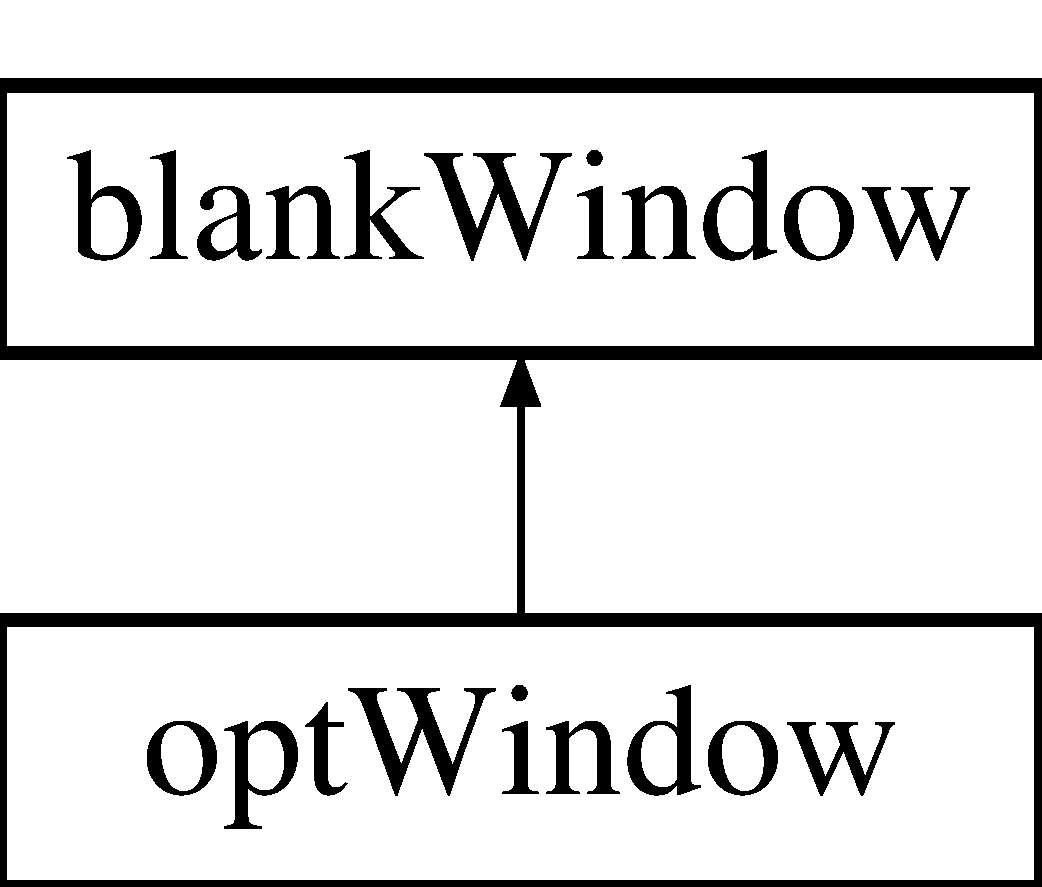
\includegraphics[height=2.000000cm]{classgui_1_1window2_1_1optWindow}
\end{center}
\end{figure}
\subsection*{\-Private \-Member \-Functions}
\begin{DoxyCompactItemize}
\item 
def \hyperlink{classgui_1_1window2_1_1optWindow_aba31902186de9c54cc3cba810c1f3634}{\-\_\-add\-File\-Menu}
\begin{DoxyCompactList}\small\item\em \-This adds a file menu to the window's menu bar. \end{DoxyCompactList}\item 
\hypertarget{classgui_1_1window2_1_1optWindow_a67ef40998197523b8ce51ec49aa57b94}{def \hyperlink{classgui_1_1window2_1_1optWindow_a67ef40998197523b8ce51ec49aa57b94}{\-\_\-add\-Help\-Menu}}\label{classgui_1_1window2_1_1optWindow_a67ef40998197523b8ce51ec49aa57b94}

\begin{DoxyCompactList}\small\item\em \-This adds the help menu to the menu bar. \end{DoxyCompactList}\item 
def \hyperlink{classgui_1_1window2_1_1optWindow_a5d355464940badfea4734a52190bfbc7}{\-\_\-check\-Opts}
\begin{DoxyCompactList}\small\item\em \-This checks which kind of options shal be set and modifies the options window in that way. \end{DoxyCompactList}\item 
def \hyperlink{classgui_1_1window2_1_1optWindow_a3d7a5345f604f41ff6563f73376434bf}{\-\_\-save\-Opts}
\begin{DoxyCompactList}\small\item\em \-This saves options into a config file. \end{DoxyCompactList}\item 
\hypertarget{classgui_1_1window2_1_1optWindow_a5d2809680f561c4d498b27120a0adbaa}{def \hyperlink{classgui_1_1window2_1_1optWindow_a5d2809680f561c4d498b27120a0adbaa}{\-\_\-close\-Window}}\label{classgui_1_1window2_1_1optWindow_a5d2809680f561c4d498b27120a0adbaa}

\begin{DoxyCompactList}\small\item\em \-This closes the options' window and reopens the main window again. \end{DoxyCompactList}\end{DoxyCompactItemize}


\subsection{\-Detailed \-Description}
\-This opens an option window where all configurations can be done. 


\begin{DoxyParams}{\-Parameters}
{\em lang} & supported language which shall be used for the \-G\-U\-I \\
\hline
{\em opts} & type of options that shall be set\-: basic, graph, output \\
\hline
{\em cfg} & this is a dictionary that holds existing configuration parameters. \\
\hline
\end{DoxyParams}


\subsection{\-Member \-Function \-Documentation}
\hypertarget{classgui_1_1window2_1_1optWindow_aba31902186de9c54cc3cba810c1f3634}{\index{gui\-::window2\-::opt\-Window@{gui\-::window2\-::opt\-Window}!\-\_\-add\-File\-Menu@{\-\_\-add\-File\-Menu}}
\index{\-\_\-add\-File\-Menu@{\-\_\-add\-File\-Menu}!gui::window2::optWindow@{gui\-::window2\-::opt\-Window}}
\subsubsection[{\-\_\-add\-File\-Menu}]{\setlength{\rightskip}{0pt plus 5cm}def {\bf \-\_\-add\-File\-Menu} (
\begin{DoxyParamCaption}
\item[{}]{self}
\end{DoxyParamCaption}
)\hspace{0.3cm}{\ttfamily  \mbox{[}private\mbox{]}}}}\label{classgui_1_1window2_1_1optWindow_aba31902186de9c54cc3cba810c1f3634}


\-This adds a file menu to the window's menu bar. 

\begin{DoxyRefDesc}{\-Todo}
\item[\hyperlink{todo__todo000015}{\-Todo}]has to be implemented \end{DoxyRefDesc}


\-References opt\-Window.\-\_\-close\-Window(), opt\-Window.\-\_\-save\-Opts(), main\-Window.\-filemenu, opt\-Window.\-filemenu, message\-Window.\-lang, blank\-Window.\-lang, main\-Window.\-lang, opt\-Window.\-lang, and blank\-Window.\-menu.

\hypertarget{classgui_1_1window2_1_1optWindow_a5d355464940badfea4734a52190bfbc7}{\index{gui\-::window2\-::opt\-Window@{gui\-::window2\-::opt\-Window}!\-\_\-check\-Opts@{\-\_\-check\-Opts}}
\index{\-\_\-check\-Opts@{\-\_\-check\-Opts}!gui::window2::optWindow@{gui\-::window2\-::opt\-Window}}
\subsubsection[{\-\_\-check\-Opts}]{\setlength{\rightskip}{0pt plus 5cm}def {\bf \-\_\-check\-Opts} (
\begin{DoxyParamCaption}
\item[{}]{self}
\end{DoxyParamCaption}
)\hspace{0.3cm}{\ttfamily  \mbox{[}private\mbox{]}}}}\label{classgui_1_1window2_1_1optWindow_a5d355464940badfea4734a52190bfbc7}


\-This checks which kind of options shal be set and modifies the options window in that way. 

\begin{DoxyRefDesc}{\-Todo}
\item[\hyperlink{todo__todo000016}{\-Todo}]has to be implemented fully \end{DoxyRefDesc}


\-References blank\-Window.\-\_\-notdoneyet(), and opt\-Window.\-opts.

\hypertarget{classgui_1_1window2_1_1optWindow_a3d7a5345f604f41ff6563f73376434bf}{\index{gui\-::window2\-::opt\-Window@{gui\-::window2\-::opt\-Window}!\-\_\-save\-Opts@{\-\_\-save\-Opts}}
\index{\-\_\-save\-Opts@{\-\_\-save\-Opts}!gui::window2::optWindow@{gui\-::window2\-::opt\-Window}}
\subsubsection[{\-\_\-save\-Opts}]{\setlength{\rightskip}{0pt plus 5cm}def {\bf \-\_\-save\-Opts} (
\begin{DoxyParamCaption}
\item[{}]{self}
\end{DoxyParamCaption}
)\hspace{0.3cm}{\ttfamily  \mbox{[}private\mbox{]}}}}\label{classgui_1_1window2_1_1optWindow_a3d7a5345f604f41ff6563f73376434bf}


\-This saves options into a config file. 

\begin{DoxyRefDesc}{\-Todo}
\item[\hyperlink{todo__todo000017}{\-Todo}]has to be implemented fully \end{DoxyRefDesc}


\-References blank\-Window.\-\_\-notdoneyet().



\-Referenced by opt\-Window.\-\_\-add\-File\-Menu(), and opt\-Window.\-\_\-close\-Window().



\-The documentation for this class was generated from the following file\-:\begin{DoxyCompactItemize}
\item 
window2.\-py\end{DoxyCompactItemize}

\chapter{\-File \-Documentation}
\hypertarget{language_8py}{\section{language.\-py \-File \-Reference}
\label{language_8py}\index{language.\-py@{language.\-py}}
}


\subsection{\-Detailed \-Description}

\hypertarget{logtools_8py}{\section{logtools.\-py \-File \-Reference}
\label{logtools_8py}\index{logtools.\-py@{logtools.\-py}}
}
\subsection*{\-Functions}
\begin{DoxyCompactItemize}
\item 
def {\bfseries mk\-Logger}
\begin{DoxyCompactList}\small\item\em \-This function builds a full usable logging object with handler. \end{DoxyCompactList}\item 
def {\bfseries create\-Logger}
\begin{DoxyCompactList}\small\item\em \-This function gets the external information of the configuration file to create the logger of it. \end{DoxyCompactList}\end{DoxyCompactItemize}
\subsection*{\-Variables}
\begin{DoxyCompactItemize}
\item 
\hypertarget{namespaceostools_1_1logtools_a1f26c4b691485aacd43d4ebc53bde938}{dictionary {\bfseries \-L\-E\-V\-E\-L}}\label{namespaceostools_1_1logtools_a1f26c4b691485aacd43d4ebc53bde938}

\begin{DoxyCompactList}\small\item\em possible log levels \end{DoxyCompactList}\end{DoxyCompactItemize}


\subsection{\-Detailed \-Description}

\hypertarget{ostools_8py}{\section{ostools.\-py \-File \-Reference}
\label{ostools_8py}\index{ostools.\-py@{ostools.\-py}}
}


\subsection{\-Detailed \-Description}

\printindex
\end{document}
